%!TEX root = ../main.tex

\section{Stability analysis of equilibrium solutions}
\label{sec:theoretical_analysis}

Under certain conditions, the electrical breakdown can develop
form small perturbations of the undamaged medium properties.
To clarify these conditions in this section we study
stability of constant solutions~$\phi(x, t) \equiv C, \; C \in [0, 1]$,
of the equation~\eqref{eq:one_dim}.

First, one has to find stationary constant solutions of~\eqref{eq:one_dim}.
From the definition~\eqref{eq:epsilon} follows the expressions for the derivatives
of~$\epsilon(\phi)$:
\begin{equation}
	\epsilon'(\phi) = \cfrac{-\epsilon_0 f'(\phi)}{(f(\phi) + \delta)^2} \tsemicolon \qquad \epsilon''(\phi) = \epsilon_0 \cfrac{2 (f'(\phi))^2 - f''(\phi)(f(\phi) + \delta)}{(f(\phi) + \delta)^3} \tpoint
	\label{eq:epsilon_derivatives}
\end{equation}

Substituting~$\phi(x, t) \equiv C$ into~\eqref{eq:one_dim} and
taking~\eqref{eq:epsilon_derivatives} into account, one has:
\begin{equation}
	f'(C) \left( \cfrac{\Gamma}{l^2} - \half K_\Phi^2 \cfrac{\epsilon_0}{(f(C) + \delta)^2} \right) = 0 \tpoint
	\label{eq:equilibrium}
\end{equation}
First, consider the case~$f'(C) = 12C^2 (1 - C) = 0$,
which leads to~$C = 0,1$. Hence, $\phi \equiv 0$ and $\phi \equiv 1$ are
equilibrium solutions.

Second, let~$C \neq 0, 1$. Then
\[
\cfrac{\Gamma}{l^2} = \cfrac{K_\Phi^2 \epsilon_0}{2 (f(C) + \delta)^2}
\quad \text{and} \quad
f(C) + \delta = K_\Phi l \sqrt{\cfrac{\epsilon_0}{2 \Gamma}}.
\]

Note that~$f(C) \in [0, 1]$ and, moreover, $f(\phi)$ is monotonically
increasing. Therefore, in case $K_\Phi l \sqrt{\epsilon_0 / (2
  \Gamma)} \in (\delta, 1 + \delta)$ the
equation~\eqref{eq:equilibrium} has a solution $C_3\ne 0,1$ given by
\begin{equation}
	C_3 = f^{-1} \left( K_\Phi l \sqrt{\cfrac{\epsilon_0}{2 \Gamma}} - \delta \right) \tpoint
	\label{eq:equilibrium_third}
\end{equation}
Otherwise the equation~\eqref{eq:equilibrium} has only two solutions.

So, the number of constant equilibrium solutions depends on the following condition
being satisfied:
\begin{equation}
	\delta^2 < \cfrac{K_\Phi^2 l^2 \epsilon_0}{2 \Gamma} < (1 + \delta)^2 \tpoint
	\label{cond:equilibriums_number}
\end{equation}
It will be shown later how the
condition~\eqref{cond:equilibriums_number} is connected with the
stability properties of the equilibrium solutions and the
equation~\eqref{eq:one_dim} itself.

Let us now procees to the stability analysis of the equilibrium solutions.

Let~$\phi(x, t)$ be a solution of~\eqref{eq:one_dim}, $\delta \phi(x,
t)$ be its perturbation.
Writing down the equation~\eqref{eq:one_dim} for the perturbed solution~$\phi
+ \delta \phi$,
after linearizing we obtain the following equation for~$\delta\phi$:
\begin{equation}
  \cfrac{1}{m} \partt{(\delta \phi)} = \left(\half K_\Phi^2 \epsilon''(\phi) + \cfrac{\Gamma}{l^2} f''(\phi) \right) \delta \phi + \half \Gamma \partxx{(\delta \phi)} \tpoint
  \label{eq:variation}
\end{equation}
For further analysis it is convenient to write~\eqref{eq:variation} as:
%
\begin{equation}
  \partt{(\delta \phi)} = A \delta \phi + B \partxx{(\delta \phi)} \tcomma
  \label{eq:variation_common}
\end{equation}
where~$A$ and~$B  > 0$ are the respective parameters.

Choosing~$\delta \phi = e^{\alpha t} \sin(\omega x)$, one obtains from~\eqref{eq:variation_common}
the following relation for the parameters of the perturbation:
$$\alpha e^{\alpha t} \sin(\omega x) = A e^{\alpha t} \sin(\omega x) - B \omega^2 e^{\alpha t} \sin(\omega x) \tcomma$$
from where follows:
\begin{equation}
  \alpha = A - B \omega^2 \tpoint
  \label{eq:exponent_coefficient}
\end{equation}

% Summing up, let us combine now the three parts of the reasoning.
% Consider equilibrium solution~$\phi \equiv C$ of the
% equation~\eqref{eq:one_dim} perturbed by~$\delta \phi$.

% ; применим к $\delta \phi$ уравнение \eqref{eq:variation}, в
% $\epsilon''$ и $f''$ подставим $\phi = C$. Полученное уравнение
% имеет вид~\eqref{eq:variation_common}.

Now it is easy to see that, depending on the value of the coefficient
$$A = \half K_\Phi^2 \epsilon''(C) + \cfrac{\Gamma}{l^2} f''(C) \tcomma$$
three cases arise:
%
\begin{enumerate}[label=\arabic*.]
\item $A > 0$. In this case, from~$\omega^2 \in [0, A / B)$ it follows
  that~$\alpha > 0$, i.e., there exists a perturbation~$\delta \phi$
  growing in time. Hence, the equilibrium solution~$\phi \equiv C$ is
  unstable.
  
\item $A < 0$. Then, for an arbitrary~$\omega$ remains~$\alpha
  \leqslant A < 0$. Next, any perturbation~$\delta \phi$ in the
  interval~$[0, W]_x$ 
  can be represented as Fourier integral over harmonics decreasing
  at least as the harmonic for~$\omega = 0$.
  Hence, the equilibrium solution~$\phi \equiv C$ is stable.
  
\item $A = 0$. Repeating the same reasoning as in the case~$A < 0$,
  one can observe that there exist arbitrarily slowly decreasing
  harmonics (i.e., harmonics with arbitrarily small values of~$\alpha$).
  This case corresponds to neutral stability of the equilibrium
  solution, and linear analysis does not provide complete
  information.
  This case will be considered in more details later.
\end{enumerate}

We now proceed to the discussion of the particular equilibrium states.

Consider the equilibrium solution~$\phi \equiv 0$.
One has~$f''(0) = 0$, $\epsilon''(0) = 0$
(see~\eqref{eq:epsilon_derivatives}),
which leads to~$A = 0$.
As it was noted before, this case requires an elaborate analysis, which will be
performed later.

Consider the equilibrium solution~$\phi \equiv 1$.
In this case~$f''(0) = -12$, $\epsilon''(0) = 12 \epsilon_0 / (1 +
\delta)^2$ (see~\eqref{eq:epsilon_derivatives}).
As a result, we obtain:
$$A = \half K_\Phi^2 \epsilon''(C) + \cfrac{\Gamma}{l^2} f''(C) = \cfrac{6 K_\Phi^2 \epsilon_0}{(1 + \delta)^2} - \cfrac{12 \Gamma}{l^2} \tpoint$$
The equilibrium state is stable if~$A < 0$, i.e., as:
\begin{equation}
  \cfrac{K_\Phi^2 l^2 \epsilon_0}{2 \Gamma} < (1 + \delta)^2 \tpoint
  \label{cond:equilibrium_1_stable}
\end{equation}      
For this case of an unstable equilibrium, let us find~$\omega_0$ such that
increasing harmonics are replaced by the decreasing ones.
To do this, consider~\eqref{eq:exponent_coefficient} with~$\alpha =
0$, $B = \Gamma/2$ and~$A$ given above to obtain: 
$$0 = \cfrac{6 K_\Phi^2 \epsilon_0}{(1 + \delta)^2} - \cfrac{12 \Gamma}{l^2} - \cfrac{\Gamma}{2} \omega_0^2 \tcomma$$
from where follows:
$$\omega_0 = 2 \sqrt{\cfrac{3 K_\Phi^2 \epsilon_0}{\Gamma (1 + \delta)^2} - \cfrac{6}{l^2}} \tpoint$$

Note that the condition~\eqref{cond:equilibrium_1_stable} is exactly the
right-hand side of the inequality~\eqref{cond:equilibriums_number}.
To explain this and to form a complete picture of what is happening,
let us look at the equilibrium solutions from a slightly different
perspective.

Solving the equation~\eqref{eq:equilibrium}, we were finding the zeros of
the function
\begin{equation}
	\chi(\phi) = \half K_\Phi^2 \epsilon'(\phi) + \cfrac{\Gamma}{l^2} f'(\phi) \tpoint
	\label{eq:equilibruim_characteristic}
\end{equation}
Hence, each equilibrium solution $\phi \equiv C$ uniquely
corresponds to a zero~$C$ of the function~$\chi(\phi)$.
From the derivation of the equation~\eqref{eq:variation} for the perturbation
it follows that in its right-hand side the coefficient at~$\delta
\phi$ is~$\chi'(\phi)$.
Later, analyzing the equation~\eqref{eq:variation_common} for an equilibrium
solution~$\phi \equiv C$, we considered several cases depending on the
sign of the coefficient~$A$, which turns out to be exactly~$\chi'(C)$.


Summing up the results, one can state the following.
The function~$\chi(\phi)$ defined by~\eqref{eq:equilibruim_characteristic}
is smooth on~$[0, 1]$ and always has zeros~$C_1=0$ and~$C_2=1$.
The third zero~$C=C_3\in (0, 1)$ exists under the
condition~\eqref{cond:equilibriums_number}.
Each equilibrium solution~$\phi \equiv C$ uniquely corresponds to a zero
of the function~$\chi(\phi)$. Their stability properties are
described in terms of the sign of~$\chi'(\phi)$ at the zeros: positive
values of~$\chi'$
correspond to the unstable solution and negative ones~---
to the stable one.

It is also clear that in the case of vanishing~$\chi'$
(as for~$\phi = 0$) the linear analysis is not enough~---
it is necessary to analyse the sign of the first higher-order
non-vanishing
derivative of~$\chi$~--- the equilibrium solution is stable if
this derivative is negative and unstable if it is positive.


Finally we show that~$\chi(\phi)$ has a non-vanishing derivative at its
zero~$C=C_3 \in (0, 1)$ (if the latter exists).
Indeed, one has:
$$\chi(C_3) = f'(C_3) \left( \cfrac{\Gamma}{l^2} - \cfrac{K_\Phi^2 \epsilon_0}{2 (f(C_3) + \delta)^2} \right) = 0 \tpoint$$
Taking into account that~$f'(C_3) \ne 0$, one obtains:
$$\cfrac{\Gamma}{l^2} - \cfrac{K_\Phi^2 \epsilon_0}{2 (f(C_3) + \delta)^2} = 0 \tpoint$$
Then:
$$\chi'(\phi)|_{C_3} = f'(C_3) \left( \cfrac{\Gamma}{l^2} - \cfrac{K_\Phi^2 \epsilon_0}{2 (f(\phi) + \delta)^2} \right) ' \bigg|_{C_3} = (f'(C_3))^2 \cfrac{K_\Phi^2 \epsilon_0}{(f(C_3) + \delta)^3} \ne 0 \tpoint$$

Now it is possible to provide a comprehensive analysis of the behavior
of~$\chi(\phi)$ at its zeros. As it can be seen from the conditions~\eqref{cond:equilibriums_number} and~\eqref{cond:equilibrium_1_stable},
its behavior is governed by the value of the parameter
\begin{equation}
  \xi = \cfrac{K_\Phi^2 l^2 \epsilon_0}{2 \Gamma} \tpoint
  \label{char:equilibriums}
\end{equation}

First, consider the case~$0 \leqslant \xi < \delta^2$. The zeros
of~$\chi(\phi)$ are~$0$ and~$1$; $\chi'(0) = 0$, $\chi'(1) < 0$.
The qualitative behavior of~$\chi(\phi)$ is shown schematically on
Fig.~\ref{fig:equilibriums_case_1}.  It can be seen that the equilibrium
solution~$\phi \equiv 0$ is unstable and~$\phi \equiv 1$ is stable.
Such case can be conventionally called the case of ``weak electric field''.
This means that with all the parameters except the electric field being fixed,
the latter is so small that even an almost completely damaged
medium with~$\phi \approx 0$ is ``healed'' over time and evolves to the
completely undamaged state~$\phi \approx 1$.

Second, consider the case~$\delta^2 < \xi < (1 + \delta)^2$.
The zeros of~$\chi(\phi)$ are $C=0$, $C=C_3$
(see~\eqref{eq:equilibrium_third}) and $C=1$; $\chi'(0) = 0, \;
\chi'(1) < 0; \; \chi'(C_3) > 0$
(since~$\chi$ is smooth).
The behavior of~$\chi(\phi)$ in this case is shown on
Fig.~\ref{fig:equilibriums_case_2}.
The equilibrium solutions are: $\phi \equiv 0$~--- stable one, $\phi
\equiv C_3$~--- unstable one, and~$\phi \equiv 1$~--- also stable.
Such case can be conventionally called the case of the ``medium
electric field''.
This means that as the values of~$\phi$ are sufficiently close to~$0$,
the damage increases, i.e.,~$\phi$ tends to zero;
as the values of~$\phi$ are sufficiently close to~$1$,
the damage decreases, i.e.,~$\phi$ tends to one;
at certain intermediate values the equilibrium is unstable.

Finally, consider the case~ $(1 + \delta)^2 < \xi$.
The zeros of~$\chi(\phi)$ are~$C=0$ and~$C=1$; $\chi'(0) = 0$, $\chi'(1)>0$.
The qualitative behavior of~$\chi(\phi)$ is schematically shown on
Fig.~\ref{fig:equilibriums_case_3}.
The equilibrium solutions are: $\phi \equiv 0$~--- the stable one, $\phi
\equiv 1$~--- the unstable one.
This case can be conventionally called the case of ``strong
electric field''.
This means that the electric field is sufficiently strong and
any state arbitrarily close to the completely undamaged one
(i.e., any state close to~$\phi \approx 1$) evolves towards
the completely damaged state~$\phi= 0$.
Essentially this is the case where the completely damaged state develops
from arbitrarily small perturbations of the completely undamaged
equilibrium solution.

In all the three cases stability of the equilibrium solution~$\phi \equiv
0$ is defined by the higher order derivatives of~$\chi(\phi)$.

\begin{figure}[!tp]
  \centering
  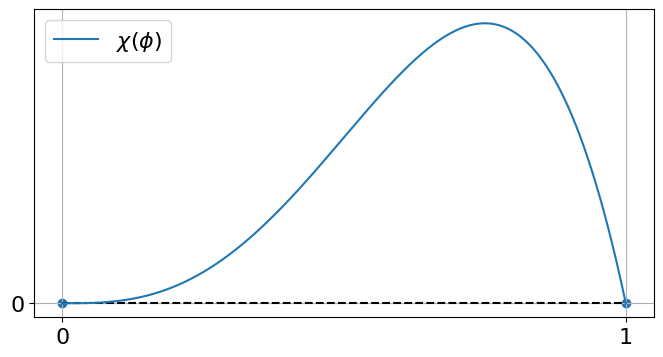
\includegraphics[width=0.84\textwidth]{figures/equilibriums_case_1.png}
  \vspace{-0.3cm}
  \caption{Characteristic behavior of~$\chi(\phi)$,
    ``weak electric field'' case.}
  \label{fig:equilibriums_case_1}
  \vspace{0.7cm}
  
  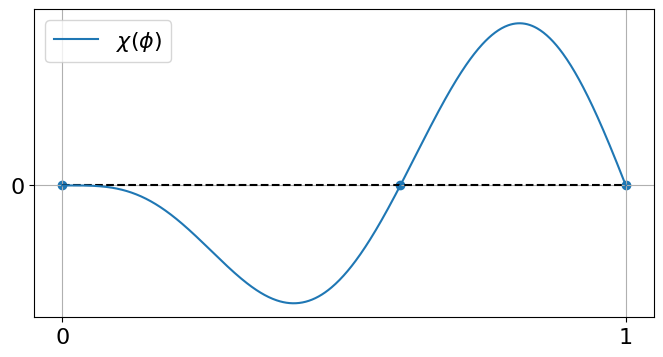
\includegraphics[width=0.84\textwidth]{figures/equilibriums_case_2.png}
  \vspace{-0.3cm}
  \caption{Characteristic behavior of~$\chi(\phi)$,
    ``medium electric field'' case.}
  \label{fig:equilibriums_case_2}
  \vspace{0.7cm}
  
  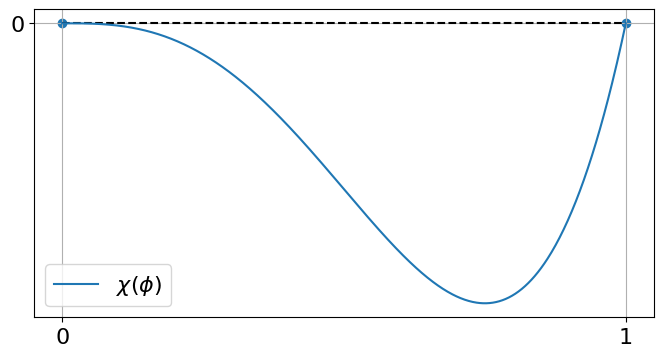
\includegraphics[width=0.84\textwidth]{figures/equilibriums_case_3.png}
  \vspace{-0.3cm}
  \caption{Characteristic behavior of~$\chi(\phi)$,
    ``strong electric field'' case.}
  \label{fig:equilibriums_case_3}
\end{figure}

% EOF